\subsection{Identity is decodable within a microphone but transfers only weakly across microphones}
Emitter identification (40 bats with positive codes; majority class 0.145, chance 0.025) with voiced features reached 0.593 (\ci{0.572}{0.618}) with random splits and 0.560 blocked by day, but 0.202 (\ci{0.115}{0.255}) when entire channels were held out (month 0.487, archive 0.504; Fig.~\ref{fig:id}). Raw accuracy is a poor yardstick for held-out channels, because predictions depend on class frequencies: balanced accuracy was 0.125 against 0.036 when emitter labels were shuffled within channel$\times$month strata (chance 0.025), so cross-channel identity information is present but weak. Normalising channels, as in earlier supervised work \cite{prat2016}, did not rescue the transfer: per-channel mean subtraction, per-channel standardisation and per-channel$\times$month subtraction gave channel-blocked balanced accuracies of 0.099, 0.088 and 0.083 (nulls 0.021, 0.017, 0.006), with the same pattern for whole-span features and syllable shapes (Supplement Table~S3). Channel itself was decodable on unseen bats (accuracy 0.63--0.85, majority 0.36). Within one channel on unseen days, however, identity was recoverable: pooled over 70 bat--channel classes accuracy was 0.648 against a within-channel majority rate of 0.326 ($+0.322$, \ci{0.288}{0.347}). For 16,663 pair-coded files, an identifier trained on positive-coded files assigned a mean probability of 0.461 to the two recognised participants (stratum-shuffle null 0.290; 0 of 100 reached it) and ranked a participant first in 58.7\% of files (null 33.1\%); trained only on other channels, 0.183 against 0.126.

\begin{figure}[!t]\centering
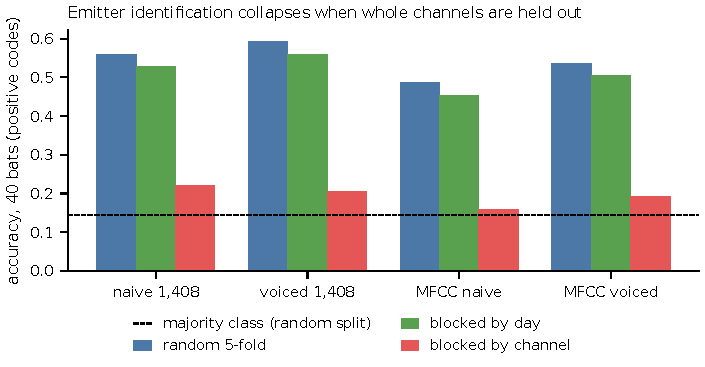
\includegraphics{fig6_v4.pdf}
\caption{Emitter identification from four representations with random, day-blocked and channel-blocked folds (41,116-file discovery sample; horizontal line: majority-class rate).}\label{fig:id}
\end{figure}

\subsection{Context, repeatability and a second dataset}
In mixed models with random intercepts for bat and channel$\times$month stratum, context remained significant for the whole-span label (likelihood-ratio $\chi^2=1{,}643$, df 12; 315 among positive-coded bats) and for a forced voiced split ($\chi^2=1{,}485$ and 366; all $p<10^{-16}$); repeatability by bat was 0.075 (\ci{0.058}{0.109}) for the whole-span label and 0.132 (\ci{0.095}{0.187}) for the voiced split. Context effects were modest (among positive-coded bats, Fighting versus General $-0.45$ logit, \ci{-0.55}{-0.35}, whole-span; Isolation versus General $+0.36$, \ci{0.31}{0.42}, voiced).

In Dataset B the microphone's FCM split (FPC 0.629) followed voiced duration (AUC 0.89) and SNR (0.90), and partitions from the microphone and the piezo agreed beyond chance for the 1,408-statistic features (ARI 0.36--0.44 at $k=2$; shuffled-pairing null 0.00) but largely not within microphone-duration quintiles (ARI 0.02--0.35), i.e.\ the shared structure is event length and loudness. The one-cluster battery gave prediction strength 0.67 (\ci{0.66}{0.85}; nulls 0.97, 0.96) for the microphone, in line with Dataset A. The piezo's two-way split, by contrast, was reproducible across individuals (prediction strength 0.93, \ci{0.82}{0.95}; nulls 0.99, 0.97) and its dip statistic exceeded the session-mean null; it was an event-length and SNR axis, and event length itself is multimodal in Dataset B (Hartigan dip of $\log_{10}$ voiced duration 0.015 and 0.012, $p<10^{-4}$) whereas SNR is unimodal. Because the dataset's authors delimited the events with their detection pipeline, we cannot tell whether this multimodality is behavioural (isolated syllables versus sequences) or procedural. Hearing status and sex were not decodable on held-out individuals (accuracy 0.44--0.59, below the majority rate).
